\section{Usability and Memorability}
  
  Authentication with text-based passwords are a common approach, but it is well known that users often choose weaker passwords because of the limitations of recalling text-based passwords. Graphical passwords came as an alternative solution for overcoming the limitations of text-based passwords, and was inspired by researchers that showed that the graphical memory of humans is particularly well-suited to remember graphical information. 
  Like text-based passwords schemes, graphical password schemes are also a knowledge-based authentication scheme, e.g. ``something you know'' that are described in the background theory. Since it all started around 1999, there have been many suggestions for graphical password schemes. When a new password scheme are proposed, there are several aspects that need to be considered. The password scheme needs to have be hard to guess, e.g. have a high entropy, as well as being easy to use.

  \begin{wrapfigure}{l}{0.35\textwidth}
    \vspace{-20pt}
    \begin{center}
      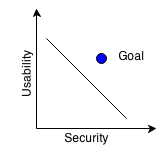
\includegraphics[scale=0.7]{pics/UsabilityVsSecurity.png}
    \end{center}
    \vspace{-20pt}
    \caption{Usability vs. Security}
    \vspace{-10pt}
  \end{wrapfigure}

   When we say that a password scheme is easy to use, it is normal to measure the success rate as well as the usability of the password scheme, e.g. how long it takes for users to remember their passwords. The problem with graphical password schemes is that they often promise improved password memorability and thus usability, while at the same time improving the security \cite{Biddle}.Since the first graphical password schemes was proposed, it is not widely in use. One of the problems with graphical approaches are that they require more overhead in the authentication phase. Like text-based passwords the users can simply type their passwords, while many of the graphical passwords require to go through many steps, requiring the user to spend more time in the authentication phase. The graphical password schemes like Passface and grIDsure are some of the graphical password schemes with commercial interest, while on mobile devices graphical passwords are not widely adopted. There is a known problem with authentication on mobile devices because of the difficulty of typing on mobile keyboards, making authentication schemes using alternatives getting increased attention. Because of the difficulty of writing on mobile keyboards it highlights the importance of understanding the usability and security implications.

  \begin{wrapfigure}{r}{0.35\textwidth}
    \vspace{-20pt}
    \begin{center}
      
\includegraphics[scale=0.35]{pics/dualCoding.png}
    \end{center}
    \vspace{-20pt}
    \caption{Dual-Coding Theory}
    \vspace{-10pt}
  \end{wrapfigure}

  In many years, the field of psychology been a important in order to understand how humans interpret and remember different information. Psychology studies have recognized that the human brain have a superior memory for recognizing and recalling visual information rather recognizing and recalling verbal or textual information. One known theory is the ``dual-coding theory'', suggesting that verbal and non-verbal memory are processed and represented differently in humans mind. Text are verbal information that is represented symbolically, in contrast to non-verbal information like images that are mentally represented in a way that perceived concepts are assigned to a perceived meaning of what is directly observed. Both verbal and non-verbal information can be used when recalling information. For example, say a person have received stimulus of the concept ``cat'', both the image of a cat as well as the word ``cat''. When the person is asked to recall the concept ``cat'', the person can retrieve the image or the word individually, or both simultaneously. If the word ``cat'' is recalled, the image of the cat is not lost and can still be retrieved at a later point in time. The ability to code a stimulus in two different ways can increase humans ability to remember, in contrast to only code the stimulus in one way. In the background theory there are described three different categories of graphical passwords according to the memory task involved in remembering and entering the password, e.g. recall, recognition and cued-recall. 

  Thorpe and Van Oorschot
